%!TEX root = alga.tex
\begin{figure}
\begin{subfigure}[b]{0.27\linewidth}
\begin{minted}[fontsize=\small]{haskell}
class Graph g where
    type Vertex g
    empty   :: g
    vertex  :: Vertex g -> g
    overlay :: g -> g -> g
    connect :: g -> g -> g
\end{minted}
\caption{The core type class}
\end{subfigure}
\hfill
\hfill
\vrule
\hfill
\hfill
\begin{subfigure}[b]{0.68\linewidth}
\begin{minted}[fontsize=\small]{haskell}
vertices     :: Graph g => [Vertex g] -> g
edge         :: Graph g => Vertex g -> Vertex g -> g
edges        :: Graph g => [(Vertex g, Vertex g)] -> g
graph        :: Graph g => [Vertex g] -> [(Vertex g, Vertex g)] -> g
gen          :: (Graph g, Arbitrary (Vertex g)) => Gen g
isSubgraphOf :: (Graph g, Eq g) => g -> g -> Bool
\end{minted}
\caption{Derived graph construction primitives and the subgraph relation}
\end{subfigure}
~\\
~\\
\begin{subfigure}[b]{0.49\linewidth}
\begin{minted}[fontsize=\small]{haskell}
domain       @\,\,@::@\,\,@Relation a -> Set a
relation     @\,\,@::@\,\,@Relation a -> Set (a, a)
adjacencyMap @\,\,@::@\,\,@AdjacencyMap a -> Map a (Set a)
adjacencyList@\,\,@::@\,\,@AdjacencyMap a -> (a, [a])
edgeList     @\,\,@::@\,\,@AdjacencyMap a -> [(a, a)]
dfsForest    @\,\,@::@\,\,@AdjacencyMap a -> Forest a
topSort      @\,\,@::@\,\,@AdjacencyMap a -> Maybe [a]
\end{minted}
\caption{Deconstructing/consuming graphs}
\end{subfigure}
\hfill
\hfill
\vrule
\hfill
\hfill
\begin{subfigure}[b]{0.47\linewidth}
\begin{minted}[fontsize=\small]{haskell}
path   @\,\,@::@\,\,@Graph@\,\,\blk{g}@ => [Vertex g] -> g
circuit@\,\,@::@\,\,@Graph@\,\,\blk{g}@ => [Vertex g] -> g
clique @\,\,@::@\,\,@Graph@\,\,\blk{g}@ => [Vertex g] -> g
star   @\,\,@::@\,\,@Graph@\,\,\blk{g}@ => Vertex g -> [Vertex g] -> g
tree   @\,\,@::@\,\,@Graph@\,\,\blk{g}@ => Tree (Vertex g) -> g
forest @\,\,@::@\,\,@Graph@\,\,\blk{g}@ => Forest (Vertex g) -> g
fold   @\,\,@::@\,\,@(Graph@\,\,\blk{g}@,@\,@Vertex@\,\,\blk{g}\,\teq@@\,\blk{a}@)@\,\,@=>@\,\,@Expr@\,\,\blk{a}\,\,@->@\,\,\blk{g}@
\end{minted}
\caption{Standard families of graphs and graph folding}
\end{subfigure}
~\\
~\\
\begin{subfigure}[b]{\linewidth}
\begin{minted}[fontsize=\small]{haskell}
transpose     :: Transpose g -> g
toList        :: ToList a -> [a]
gmap          :: Graph g => (a -> Vertex g) -> GraphFunctor a -> g
mergeVertices :: Graph g => (Vertex g -> Bool) -> Vertex g -> GraphFunctor (Vertex g) -> g
bind          :: Graph g => GraphMonad a -> (a -> g) -> g
induce        :: Graph g => (Vertex g -> Bool) -> GraphMonad (Vertex g) -> g
removeVertex  :: (Graph g, Eq (Vertex g)) => Vertex g -> GraphMonad (Vertex g) -> g
splitVertex   :: (Graph g, Eq (Vertex g)) => Vertex g -> [Vertex g] -> GraphMonad (Vertex g) -> g
removeEdge    :: (Graph g, Eq (Vertex g)) => Vertex g -> Vertex g -> GraphMonad (Vertex g) -> g
box           :: (Graph g, Vertex g @\teq@ (u, v)) => GraphFunctor u -> GraphFunctor v -> g
deBruijn      :: (Graph g, Vertex g @\teq@ [a]) => Int -> [a] -> g
\end{minted}
\caption{Polymorphic graph transformations}
\end{subfigure}
\vspace{-3mm}
\caption{API of the graph transformation library\label{fig-api}}
\end{figure}

\newpage
\section{Graph transformation library}\label{sec-transformations}

In this section we demonstrate the flexibility of the algebraic graph core,
and develop a graph transformation library whose API is summarised in
Fig.~\ref{fig-api}. The parts of the API shown in Fig.~\ref{fig-api}(a-c)
were defined in~\S\ref{sec-algebra} and~\S\ref{sec-a-la-carte}.

\subsection{Standard families of graphs}\label{sub-families}

This subsection defines a few simple functions for constructing graphs from
standard graph families. An example is the family of \emph{clique} graphs that has
already been covered in \S\ref{sec-algebra}, where we defined the function
\hs{clique}. See Fig.~\ref{fig-api}(d) for the list of all functions we define.

A \emph{path} on a list of vertices can be constructed from the \hs{edges}
formed by the path neighbours:

\begin{minted}{haskell}
path :: Graph g => [Vertex g] -> g
path []  = empty
path [x] = vertex x
path xs  = edges $ @\std{zip}@ xs (@\std{tail}@ xs)
\end{minted}

\noindent
Note that the case with a single vertex on the path requires a special treatment.

If we connect the last vertex of a path to the first one, we get a \emph{circuit}
graph, or a \emph{cycle}. Let's express this in terms of the \hs{path} function:

\begin{minted}{haskell}
circuit :: Graph g => [Vertex g] -> g
circuit []     = empty
circuit (x:xs) = path $ [x] ++ xs ++ [x]
\end{minted}

A \emph{star} graph can be obtained by connecting a centre vertex to a given
list of \emph{leaves}:

\begin{minted}{haskell}
star :: Graph g => Vertex g -> [Vertex g] -> g
star x ys = connect (vertex x) (vertices ys)
\end{minted}

Finally, \emph{trees} and \emph{forests} can be constructed by the following
pair of mutually recursive functions:

\begin{minted}{haskell}
tree :: Graph g => Tree (Vertex g) -> g
tree (Node r f) = overlay (star r $ @\std{map}@ rootLabel f) (forest f)

forest :: Graph g => Forest (Vertex g) -> g
forest = @\std{foldr}@ overlay empty . @\std{map}@ tree
\end{minted}

\noindent
That is, a tree is represented by a star overlaid with the forest
of subtrees of the root's descendants. We remind the reader the
definitions of the data types \hs{Tree} and \hs{Forest} from the
\textsf{containers} library for completeness:

\begin{minted}{haskell}
data Tree a = Node { rootLabel :: a, subForest :: Forest a }

type Forest a = [Tree a]
\end{minted}

Below we experiment with these functions and their properties, and define
graphs \hs{pentagon} and \hs{p4} that will be used in subsection~\S\ref{sub-functor}
and in particular will feature in Fig.~\ref{fig-product}.

\begin{minted}[frame=single]{haskell}
@\ghci@ pentagon = circuit [1..5]
@\ghci@ p4 = path "abcd"

@\ghci@ :t pentagon
@\blk{pentagon}@ :: (Graph g, Num (Vertex g), Enum (Vertex g)) => g

@\ghci@ edgeList p4
[('a','b'),('b','c'),('c','d')]

@\ghci@ quickCheck $ \xs -> path xs `isSubgraphOf` (circuit xs :: Relation Int)
@\blk{+++ OK, passed 100 tests.}@

@\ghci@ adjacencyList $ forest $ dfsForest (1 + 2 * 3 + 4 * (5 + 6))
[(1,[@@]),(2,[3]),(3,[@@]),(4,[5,6]),(5,[@@]),(6,[@@])]

@\ghci@ quickCheck $ \xs -> path xs == (clique xs :: Transitive Int)
@\blk{+++ OK, passed 100 tests.}@
\end{minted}

The last property deserves a remark: the transitive closure of a path graph
is the clique on the same set of vertices, therefore they are considered equal
when interpreted by the \hs{Transitive} graph instance.

\subsection{Graph transpose}

In the rest of this section we present a toolbox for transforming polymorphic graph
expressions without turning them into a concrete data structure. The functions of the
presented toolbox are listed in Fig.~\ref{fig-api}(e).

One of the simplest transformations one can apply to a graph is to flip the
direction of all of its edges. It's usually straightforward to implement but
whatever data structure you use to represent graphs, you will spend at least
$O(1)$ time to modify it (say, by flipping the \hs{treatAsTransposed} flag);
much more often you will have to traverse the data structure and flip every edge,
resulting in $O(|V|+|E|)$ time complexity. However, by working with polymorphic
graphs, i.e. graphs of type \hs{forall g. Graph g => g}, and using Haskell's
zero-cost \hs{newtype} wrappers, we can implement transpose that takes zero time.

Consider the following \hs{Graph} instance:

\begin{minted}{haskell}
newtype Transpose g = T { transpose :: g } deriving (Arbitrary, Eq, Show)
\end{minted}
\vspace{1mm}
\begin{minted}{haskell}
instance Graph g => Graph (Transpose g) where
    type Vertex (Transpose g) = Vertex g
    empty       = T empty
    vertex      = T . vertex
    overlay x y = T $ overlay (transpose x) (transpose y)
    connect x y = T $ connect (transpose y) (transpose x) -- flip it!
\end{minted}

\noindent
That is, we wrap a graph in a \hs{newtype} flipping the order of \hs{connect} arguments.
Let's check if this works:

\begin{minted}[frame=single]{haskell}
@\ghci@ edgeList $ 1 * (2 + 3) * 4
[(1,2),(1,3),(1,4),(2,4),(3,4)]

@\ghci@ edgeList $ transpose $ 1 * (2 + 3) * 4
[(2,1),(3,1),(4,1),(4,2),(4,3)]
\end{minted}

This has zero runtime cost, because all we do is wrapping and unwrapping
the \hs{newtype}, which is guaranteed to be free or, more precisely, is handled
by the GHC at the compile time.

To make sure \hs{transpose} is only applied to polymorphic graphs, we do not export
the constructor \hs{T}, therefore the only way to call \hs{transpose} is to give it a
polymorphic argument and let the type inference interpret it as a value of type
\hs{Transpose}.

\subsection{Graph functor}\label{sub-functor}

We now implement a function \hs{gmap} that given a function \hs{a}~\hs{->}~\hs{b}
and a polymorphic graph whose vertices are of type \hs{a} will produce a
polymorphic graph with vertices of type \hs{b} by applying the function
to each vertex. This is almost a \hs{Functor} but it does not have the usual
type signature, because \hs{Graph} is not a higher-kinded type:

\vspace{2mm}
\begin{minted}{haskell}
newtype GraphFunctor a = GF { gfor :: forall g. Graph g => (a -> Vertex g) -> g }
\end{minted}
\vspace{1mm}
\begin{minted}{haskell}
instance Graph (GraphFunctor a) where
    type Vertex (GraphFunctor a) = a
    empty       = GF $ \_ -> empty
    vertex  x   = GF $ \f -> vertex (f x)
    overlay x y = GF $ \f -> overlay (gmap f x) (gmap f y)
    connect x y = GF $ \f -> connect (gmap f x) (gmap f y)
\end{minted}
\vspace{1mm}
\begin{minted}{haskell}
gmap :: Graph g => (a -> Vertex g) -> GraphFunctor a -> g
gmap = flip gfor
\end{minted}

Essentially, we are defining another newtype wrapper, which pushes the
given function all the way towards the vertices. This has no runtime cost,
just as before, although the actual evaluation of the given function at each
vertex will not be free, of course. Let's test this:

\begin{minted}[frame=single]{haskell}
@\ghci@ adjacencyList $ 1 * 2 * 3 + 4 * 5
[(1,[2,3]),(2,[3]),(3,[@@]),(4,[5]),(5,[@@])]

@\ghci@ adjacencyList $ gmap (+1) $ 1 * 2 * 3 + 4 * 5
[(2,[3,4]),(3,[4]),(4,[@@]),(5,[6]),(6,[@@])]
\end{minted}
\vspace{-1mm}
As you can see, we can increment the value of each vertex by mapping the function
\hs{(+1)} over the graph. The resulting expression is a polymorphic graph, as desired.
Again, we have done some useful work without turning the graph into a concrete data
structure. Note that \hs{gmap} satisfies the usual functor laws
\hs{gmap id = id} and \hs{gmap f@ . @}\hs{gmap g@ = @}\hs{gmap (f . g)}, because
it does not change the structure of the given graph expression and only pushes
the given function down to its leaves -- the vertices.

An alert reader might wonder: what happens if the function maps two different
vertices into the same one? They will be merged! Merging graph vertices is
a useful graph transformation, so let's define it in terms of \hs{gmap}:

\begin{minted}{haskell}
mergeVertices :: Graph g => (Vertex g -> Bool) -> Vertex g -> GraphFunctor (Vertex g) -> g
mergeVertices p v = gmap $ \u -> if p u then v else u
\end{minted}
\vspace{-1mm}
\begin{minted}[frame=single]{haskell}
@\ghci@ adjacencyList $ mergeVertices odd 3 $ 1 * 2 * 3 + 4 * 5
[(2,[3]),(3,[2,3]),(4,[3])]
\end{minted}
\vspace{-1mm}
The function takes a predicate on graph vertices and a target vertex and
maps all vertices satisfying the predicate into the target, thereby
merging them. In our example the \hs{odd} vertices $\{1, 3, 5\}$ are merged
into~3, in particular creating the self-loop $3 \rightarrow 3$. Note: it takes
linear time $O(|g|)$ for \hs{mergeVertices} to apply the predicate to each vertex
(where $|g|$ is the size of the graph expression $g$), which may be much more efficient
than merging vertices in a concrete data structure. For example, if the graph
is represented by an adjacency matrix, it will likely be necessary to rebuild
the resulting matrix from scratch, which takes $O(|V|^2)$ time. Since for
many graphs we have $|g| = O(|V|)$, our \hs{mergeVertices}
may be quadratically faster than the matrix-based one.

\begin{figure}
\centerline{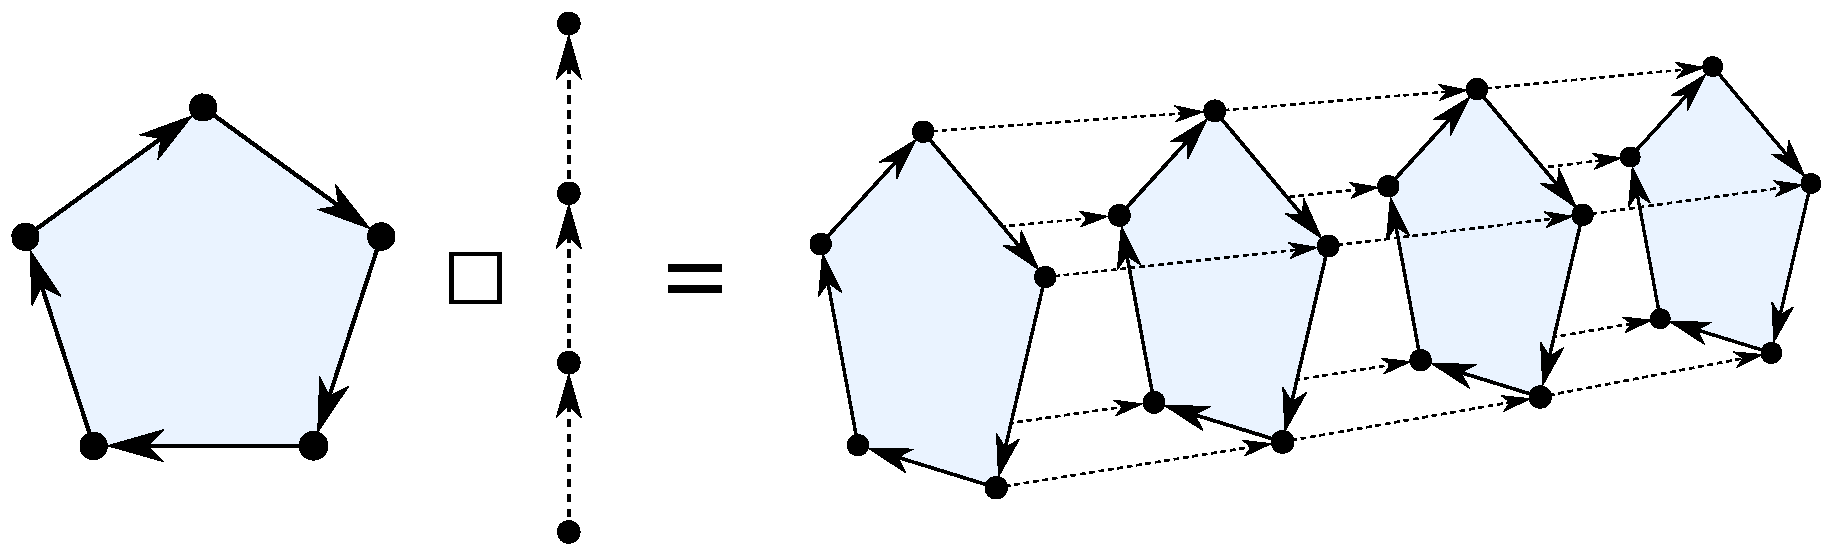
\includegraphics[scale=0.36]{fig/graph-product.pdf}}
\vspace{-4mm}
\caption{The Cartesian graph product of \hs{pentagon} and \hs{p4}, i.e. the graph
\hs{box@\,\,@}\hs{pentagon@\,\,@}\hs{p4}\label{fig-product}}
\vspace{-3mm}
\end{figure}

As another application of \hs{gmap}, we implement the \emph{Cartesian graph
product} operation \hs{box}, or $G~~\square~~H$, where the resulting vertex set is
$V_G \times V_H$ and vertex $(x, y)$ is connected to vertex $(x', y')$ if
either $x = x'$ and $(y, y') \in E_H$, or $y = y'$ and $(x,x')\in E_G$. An example of the Cartesian product of graphs \hs{pentagon}
and \hs{p4} is shown in Fig.~\ref{fig-product}.

\begin{minted}{haskell}
box :: (Graph g, Vertex g @\teq@ (u, v)) => GraphFunctor u -> GraphFunctor v -> g
box x y = @\std{foldr}@ overlay empty $ xs ++ ys
  where
    xs = @\std{map}@ (\b -> gmap (,b) x) . toList $ gmap id y
    ys = @\std{map}@ (\a -> gmap (a,) y) . toList $ gmap id x
\end{minted}

The Cartesian product $G~~\square~~H$ is assembled by creating $|V_H|$ copies
of graph $G$ and overlaying them with $|V_G|$ copies of graph $H$. We get
access to the list of graph vertices using \hs{toList} and turn vertices of
original graphs into pairs of vertices by \hs{gmap}. Note that we need to
\emph{reinterpret} the input of type \hs{GraphFunctor} as a polymorphic graph
by \hs{gmap@\,id@} before passing it to the \hs{toList} function, which expects
inputs of type \hs{ToList}. As you can see, we managed to implement quite
a sophisticated graph transformation function \hs{box} fully polymorphically.

The \hs{toList} function can be implemented by the following simple \hs{newtype}
wrapper:

\begin{minted}{haskell}
newtype ToList a = TL { toList :: [a] } deriving Show
\end{minted}
\vspace{1mm}
\begin{minted}{haskell}
instance Graph (ToList a) where -- note the lack of Eq a constraint
     type Vertex (ToList a) = a
     empty       = TL $ [@@]
     vertex  x   = TL $ [x]
     overlay x y = TL $ toList x ++ toList y
     connect x y = TL $ toList x ++ toList y
\end{minted}

\noindent
Note that we do not provide the \hs{Eq} instance for \hs{ToList}, because it
is impossible to make it law-abiding without requiring \hs{Eq} for vertices,
and we would like to avoid this in order to keep the \hs{box} type signature
fully parametric. As a consequence, \hs{toList (1 + 1)} produces the
list \hs{[1,1]}.

\subsection{Graph monad}\label{sub-monad}

What do the operations of removing a vertex and splitting a vertex have in common?
They both can be implemented by replacing each vertex of a graph with a (possibly empty)
subgraph and flattening the result. You may recognise this as monad's
\hs{bind} operation. We are going to implement \hs{bind}
by wrapping it into yet another \hs{newtype}:

\begin{minted}{haskell}
newtype GraphMonad a = GM { bind :: forall g. Graph g => (a -> g) -> g }
\end{minted}
\vspace{1mm}
\begin{minted}{haskell}
instance Graph (GraphMonad a) where
    type Vertex (GraphMonad a) = a
    empty       = GM $ \_ -> empty
    vertex  x   = GM $ \f -> f x -- here is the difference from gmap
    overlay x y = GM $ \f -> overlay (bind x f) (bind y f)
    connect x y = GM $ \f -> connect (bind x f) (bind y f)
\end{minted}

As you can see, the implementation is almost identical to \hs{gmap}: instead of
wrapping the value \hs{f@\,\,@x} into a \hs{vertex}, we should just leave it as is.
Let's see how we can make use of this new type in our toolbox.

Firstly, we are going to implement a \hs{@\std{filter}@}-like function \hs{induce}
that, given a vertex predicate and a graph, will compute the \emph{induced subgraph}
on the set of vertices that satisfy the predicate by turning all other
vertices into empty subgraphs and flattening the result.

\begin{minted}{haskell}
induce :: Graph g => (Vertex g -> Bool) -> GraphMonad (Vertex g) -> g
induce p g = bind g $ \v -> if p v then vertex v else empty
\end{minted}
\vspace{1mm}
\begin{minted}[frame=single]{haskell}
@\ghci@ edgeList $ clique [0..4]
[(0,1),(0,2),(0,3),(0,4),(1,2),(1,3),(1,4),(2,3),(2,4),(3,4)]

@\ghci@ edgeList $ induce (<3) $ clique [0..4]
[(0,1),(0,2),(1,2)]
\end{minted}

\noindent
As you can see, by inducing a clique on a subset of the vertices
that we like \hs{(<3)}, we get a smaller clique, as expected.
The cost of \hs{induce} for a given expression $g$ is $O(|g|)$.

We can now -- at last -- implement the \hs{removeVertex} function, as
was promised in the motivation section~\S\ref{sec-motivation}.

\begin{minted}{haskell}
removeVertex :: (Graph g, Eq (Vertex g)) => Vertex g -> GraphMonad (Vertex g) -> g
removeVertex v = induce (/= v)
\end{minted}
\vspace{1mm}
\begin{minted}[frame=single]{haskell}
@\ghci@ adjacencyList $ removeVertex 2 $ 1 * 2 + 3 * 1
[(1,[@@]),(3,[1])]
\end{minted}

\noindent
Note that the above example matches the one in Fig.~\ref{fig-example}.

The polymorphic implementation of \hs{removeVertex} presented above takes
$O(|g|)$ to remove a vertex from a graph expression $g$, which is
slower than some concrete data structures.

We can also use the \hs{bind} function to split a vertex into a list of given vertices:

\begin{minted}{haskell}
splitVertex :: (Graph@\,\,g@,@\,@Eq@\,@(Vertex@\,\,g@)) => Vertex@\,\,g@ -> [Vertex@\,\,g@] -> GraphMonad@\,@(Vertex@\,\,g@) -> g
splitVertex v vs g = bind g $ \u -> if u == v then vertices vs else vertex u
\end{minted}
\vspace{1mm}
\begin{minted}[frame=single]{haskell}
@\ghci@ adjacencyList $ splitVertex 1 [0, 1] $ 1 * (2 + 3)
[(0,[2,3]),(1,[2,3]),(2,[@@]),(3,[@@])]
\end{minted}

\noindent
Here vertex 1 is split into a pair of vertices $\{0, 1\}$ that have the same connectivity.

\subsection{Beyond homomorphisms}\label{sub-beyond}

Most of the \hs{newtype} wrappers defined in this section are \emph{homomorphisms},
that is, they preserve the structure of the original graph expression. The two
exceptions are: \hs{Transpose}, which is an \emph{antihomomorphism}, and
\hs{ToList} which collapses the structure of the original expression into a list.

Below we derive an implementation for \hs{removeEdge}, which is another
example of a useful function that is not a homomorphism. Removing an edge sounds
easy, but the result is the most complicated \hs{newtype} in this paper.

\begin{minted}{haskell}
newtype RemoveEdge a = RE { re :: forall g. (Vertex g @\teq@ a, Graph g) => a -> a -> g }
\end{minted}
\vspace{1mm}
\begin{minted}{haskell}
instance Eq a => Graph (RemoveEdge a) where
    type Vertex (RemoveEdge a) = a
    empty       = RE $ \_ _ -> empty
    vertex  x   = RE $ \_ _ -> vertex x
    overlay x y = RE $ \u v -> overlay (re x u v) (re y u v)
    connect x y = RE $ \u v -> connect (removeVertex u $ re x u u) (re y u v) `overlay`
                               connect (re x u v) (removeVertex v $ re y v v)
\end{minted}
\vspace{0mm}
\begin{minted}{haskell}
removeEdge :: (Eq@\,@(Vertex g),@\,@Graph g) => Vertex g -> Vertex g -> RemoveEdge@\,@(Vertex g) -> g
removeEdge u v g = re g u v
\end{minted}

\noindent
Here is how it works. Removing an edge $(u,v)$ from the \hs{empty} graph
or a \hs{vertex} is easy:
nothing needs to be done, because there are no edges. To remove the edge from an
\hs{overlay}, we simply recurse to both subexpressions, because the overlay does not create
any edges. The \hs{connect} case $x \rightarrow y$ is handled by overlaying two graphs:
$x_u \rightarrow y_{uv}$ and $x_{uv} \rightarrow y_v$, where:

\begin{itemize}
    \item $x_u = \hs{removeVertex}~u~x$ and $y_{uv} = \hs{removeEdge}~u~v~y$,
    therefore $x_u \rightarrow y_{uv}$ definitely does not contain the edge $(u,v)$
    at the cost of losing the vertices $u$ in the left-hand side $x_u$.
    \item $y_v = \hs{removeVertex}~v~y$ and $x_{uv} = \hs{removeEdge}~u~v~x$,
    therefore $x_{uv} \rightarrow y_v$ definitely does not contain the edge $(u,v)$
    at the cost of losing the vertices $v$ in the right-hand side $y_v$.
\end{itemize}
\noindent
The overlay $x_u \rightarrow y_{uv} + x_{uv} \rightarrow y_v$ restores the missing
vertices, because their copy is present in one of the subexpressions, but the
edge $(u,v)$ is removed in both subexpressions and is therefore not restored.

We demonstrate \hs{removeEdge} on two simple examples:
\begin{minted}[frame=single]{haskell}
@\ghci@ edgeList $ path "Hello"
[('H','e'),('e','l'),('l','l'),('l','o')]

@\ghci@ edgeList $ removeEdge 'H' 'e' $ path "Hello"
[('e','l'),('l','l'),('l','o')]

@\ghci@ edgeList $ removeEdge 'l' 'l' $ path "Hello"
[('H','e'),('e','l'),('l','o')]
\end{minted}

\begin{figure}
\centerline{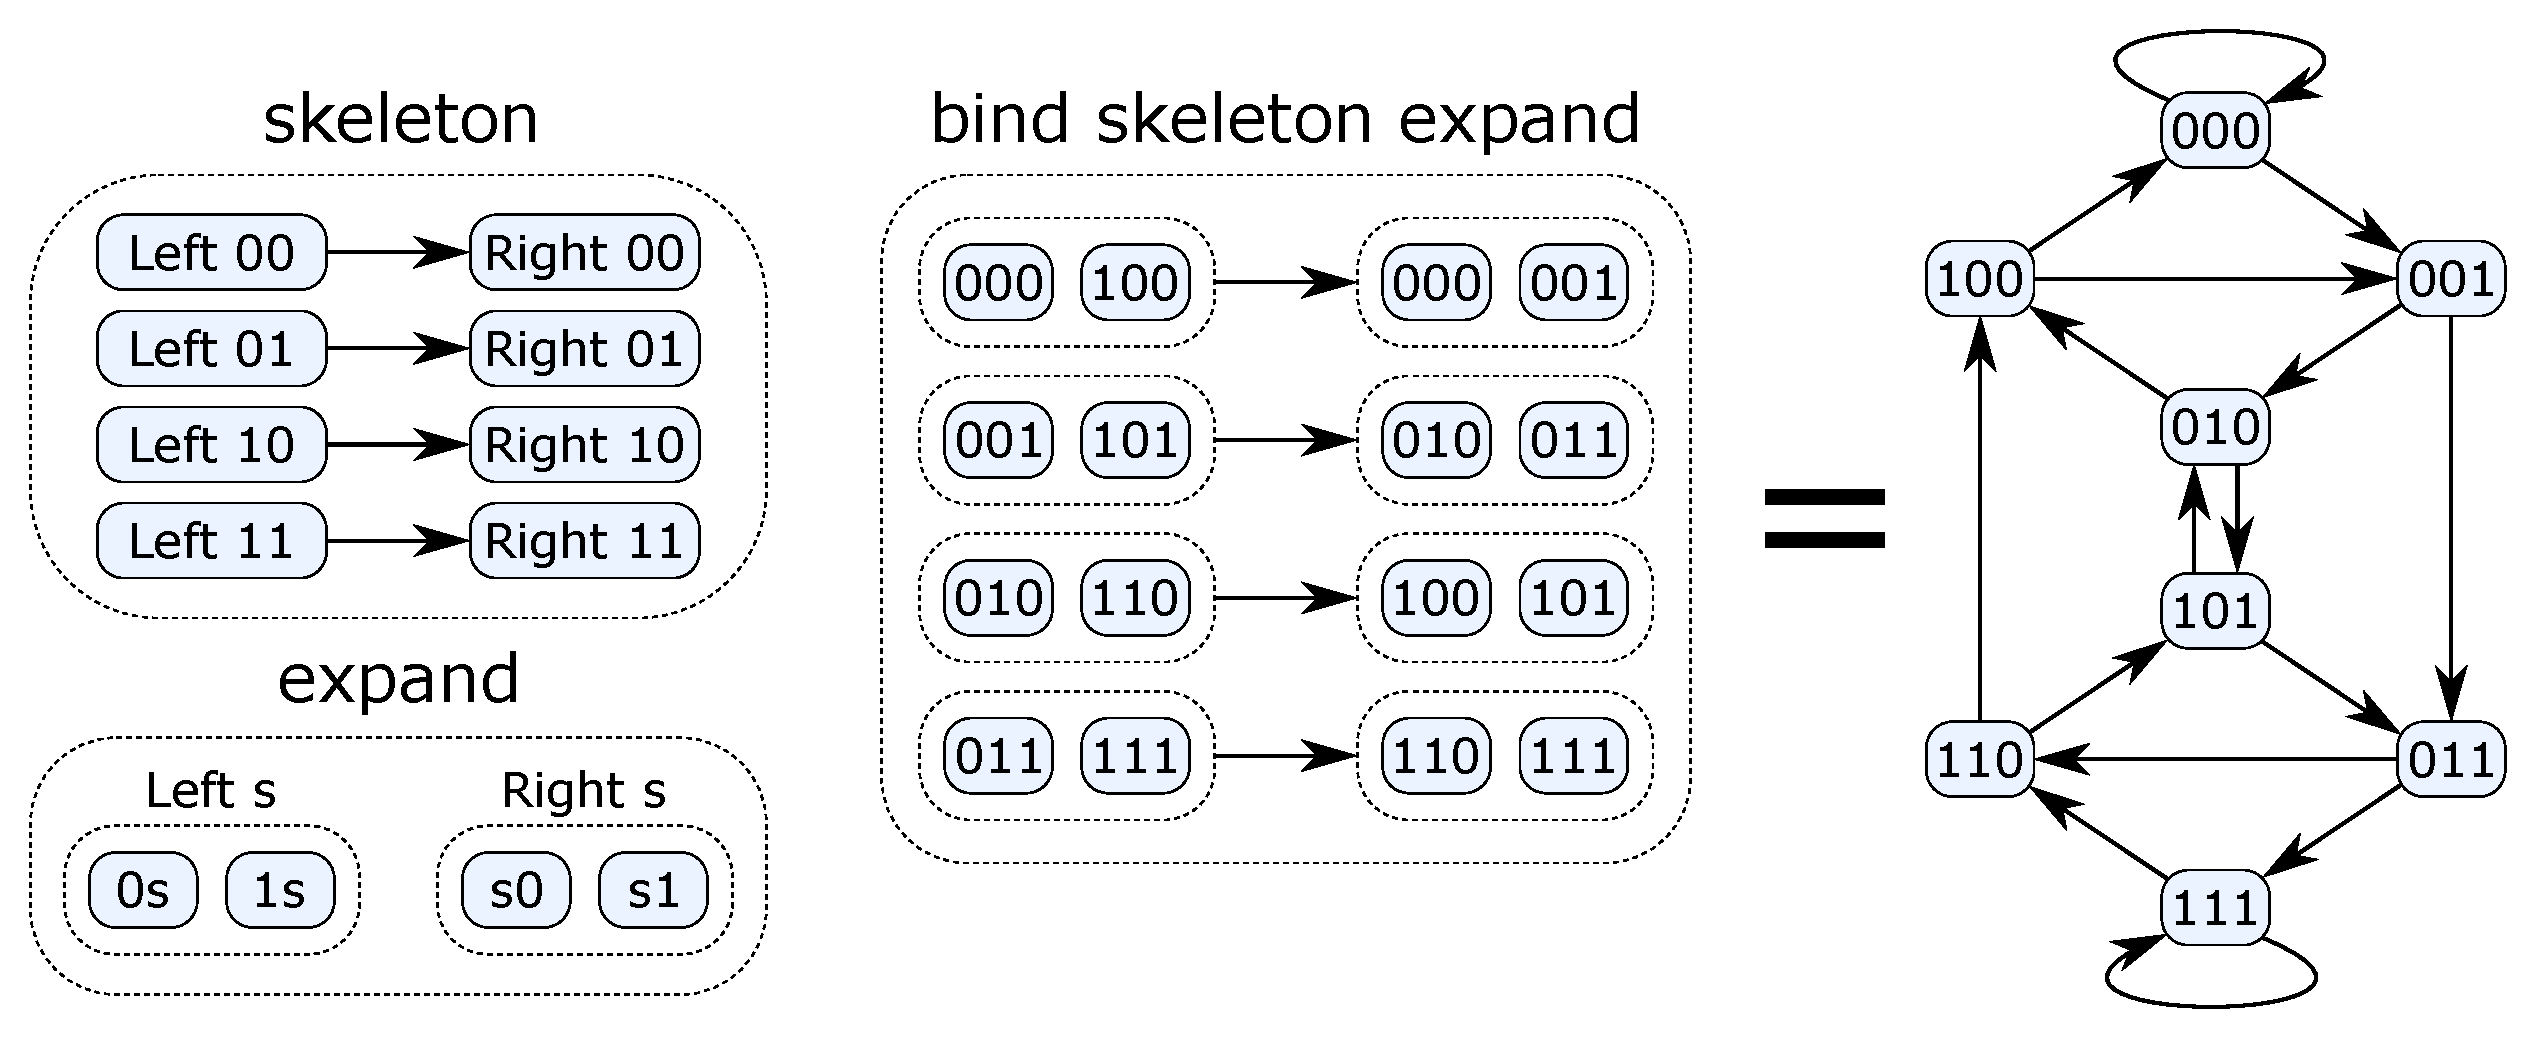
\includegraphics[scale=0.3]{fig/De-Bruijn-construction.pdf}}
\vspace{-4mm}
\caption{Constructing De Bruijn graphs\label{fig-de-bruijn}}
\vspace{-4mm}
\end{figure}


\subsection{De Bruijn graphs}

To convince the reader that we can construct reasonably sophisticated graphs using
the presented library, let's try it on \emph{De Bruijn graphs}, an interesting
combinatorial object that frequently shows up in computer engineering and
bioinformatics. The implementation is very short, but requires some explanation:

\begin{minted}{haskell}
deBruijn :: (Graph g, Vertex g @\teq@ [a]) => Int -> [a] -> g
deBruijn len alphabet = bind skeleton expand
  where
    overlaps = @\std{mapM}@ (@\std{const}@ alphabet) [2..len]
    skeleton = edges    [        (Left s, Right s)   | s <- overlaps ]
    expand v = vertices [ @\std{either}@ ([a] ++) (++ [a]) v | a <- alphabet ]
\end{minted}

The function builds a De Bruijn graph of dimension \hs{len} from symbols of the given
\hs{alphabet}. The vertices of the graph are all possible words of length \hs{len}
containing symbols of the \hs{alphabet}, and two words are connected $x \rightarrow y$
whenever $x$ and $y$ match after we remove the first symbol of $x$ and the last symbol
of $y$ (equivalently, when $x = az$ and $y = zb$ for some symbols $a$ and $b$).
The process of construction of a 3-dimensional De Bruijn graph on the alphabet
$\{0, 1\}$ is illustrated in Fig.~\ref{fig-de-bruijn}. Here are all the ingredients
of the solution:
\begin{itemize}
    \item \hs{overlaps} contains all possible words of length \hs{len-1} that
    correspond to overlaps of connected vertices.
    \item \hs{skeleton} contains one edge per overlap, with \hs{Left} and
    \hs{Right} vertices acting as temporary placeholders.
    \item We replace a vertex \hs{Left@\,$s$@} with a subgraph of two vertices
    $\{0s, 1s\}$, i.e. the vertices whose suffix is $s$. Symmetrically,
    \hs{Right@\,$s$@} is replaced by a vertices $\{s0, s1\}$. This is captured
    by the function \hs{expand}.
    \item The result is obtained by computing \hs{bind skeleton expand}.
\end{itemize}




\subsection{Benchmarks}\label{sub-benchmarks}

